\documentclass[11pt]{article}

% ---------- Packages ----------
\usepackage[a4paper,margin=1in]{geometry}
\usepackage{amsmath,amssymb,amsthm,mathtools}
\usepackage{bbm}
\usepackage{hyperref}
\usepackage{tikz}
\usetikzlibrary{arrows.meta,positioning}

% ---------- Theorem environments ----------
\newtheorem{theorem}{Theorem}
\newtheorem{definition}{Definition}
\newtheorem{lemma}{Lemma}
\newtheorem{proposition}{Proposition}
\newtheorem{corollary}{Corollary}
\newtheorem{remark}{Remark}

% ---------- Commands ----------
\newcommand{\Qcal}{\mathcal{Q}}
\newcommand{\Pcal}{\mathcal{P}}

\title{
Predictive Operator Theory for Observable Dynamical Systems
}

\author{Patrick S. Mahon}

\date{}

\begin{document}

\maketitle

\begin{abstract}
This paper develops the operator theory of predictive dynamics
arising from observable experiments.  The predictive factorization
theorem of the preceding paper forces conditional expectations of future
observables to factor through a minimal predictive state space $Q_*$.
This paper shows that predictive evolution on $O_{Q_*}$ is represented
by a strongly continuous semigroup of Markov operators $\{K_t\}_{t\ge0}$,
studies its infinitesimal generator, and situates the construction
within classical Koopman and Markov operator theory.
\end{abstract}

\section{Introduction}

This paper studies the dynamical structure that emerges from prediction
in observable systems.

The observational program of the preceding works establishes the chain
\[
\text{observable experiments}
\;\rightarrow\;
\text{probability}
\;\rightarrow\;
\text{predictive state}
\;\rightarrow\;
\text{operator dynamics}.
\]
The preceding papers construct the canonical experiment $(\Omega,\sigma(\Qcal),P)$
and the minimal predictive query $Q_*:\Omega\to O_{Q_*}$ whose states
correspond exactly to distinct predictive laws.  Because the predictive
law factors through $Q_*$, conditional expectations of future observables
define operators acting on functions of the predictive state; the present
paper is a study of those operators and their dynamical structure.

For each prediction horizon $t\ge0$, define the predictive operator by
\[
(K_t g)(q)
=
E[g(F_t)\mid Q_*=q].
\]
The central result (Theorem~\ref{thm:semigroup}) is that the family
$\{K_t\}_{t\ge0}$ forms a Markov operator semigroup on $O_{Q_*}$,
from which an infinitesimal generator and predictive Kolmogorov
equation follow by standard $C_0$-semigroup theory.
Figure~\ref{fig:paper3-spine} summarises the derivational structure
of the paper.

\begin{figure}[h]
\centering
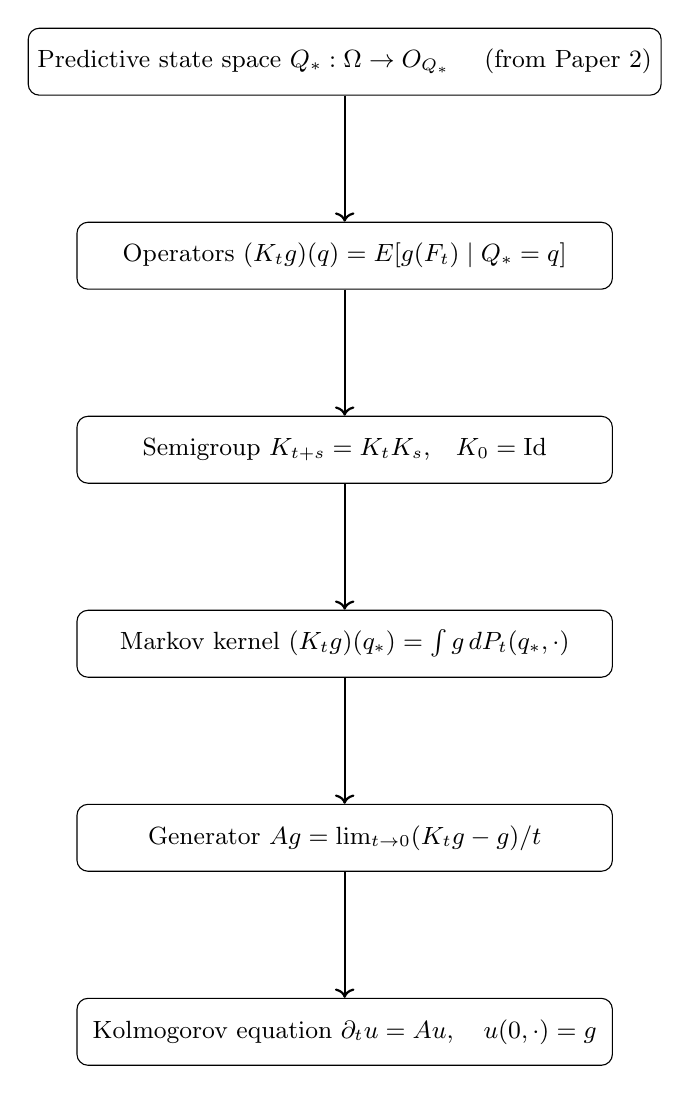
\begin{tikzpicture}[
    node distance=1.6cm,
    box/.style={
        rectangle, draw, rounded corners,
        minimum width=6.8cm, minimum height=0.85cm,
        align=center, font=\small
    },
    arrow/.style={->,thick}
]
\node[box] (state)  {Predictive state space $Q_*:\Omega\to O_{Q_*}$
                     \quad\textnormal{(from Paper 2)}};
\node[box,below=of state] (ops)
    {Operators $(K_t g)(q)=E[g(F_t)\mid Q_*=q]$};
\node[box,below=of ops]   (sg)
    {Semigroup $K_{t+s}=K_t K_s$,\quad $K_0=\mathrm{Id}$};
\node[box,below=of sg]    (ker)
    {Markov kernel $(K_t g)(q_*)=\int g\,dP_t(q_*,\cdot)$};
\node[box,below=of ker]   (gen)
    {Generator $Ag=\lim_{t\to0}(K_t g-g)/t$};
\node[box,below=of gen]   (kolm)
    {Kolmogorov equation $\partial_t u=Au,\quad u(0,\cdot)=g$};

\draw[arrow] (state) -- (ops);
\draw[arrow] (ops)   -- (sg);
\draw[arrow] (sg)    -- (ker);
\draw[arrow] (ker)   -- (gen);
\draw[arrow] (gen)   -- (kolm);
\end{tikzpicture}
\caption{Derivational structure of Paper 3.}
\label{fig:paper3-spine}
\end{figure}

\paragraph{Structure of the paper.}
Section~\ref{sec:framework} fixes the standing framework.
Section~\ref{sec:operators} defines the predictive operators and
establishes basic positivity properties.
Section~\ref{sec:semigroup} proves the semigroup theorem and the
Markov kernel representation.
Section~\ref{sec:generator} defines the infinitesimal generator and
derives the predictive Kolmogorov equation.
Section~\ref{sec:koopman} situates the construction within classical
Koopman and Markov operator theory.
Sections~\ref{sec:spectral}--\ref{sec:empirical} address spectral
structure, the observable dynamical system, and empirical approximation.

\section{Standing framework}\label{sec:framework}

The following objects are assumed throughout.

\begin{itemize}
\item A query system $(\Qcal,\preceq)$ and canonical experiment $(\Omega,\sigma(\Qcal),P)$.
\item The minimal predictive query $Q_*:\Omega \to O_{Q_*}$, whose states
      correspond exactly to distinct predictive laws.
\item A parametrized family of future observables $F_t:\Omega\to O_F$,
      $t\ge0$, with $O_F$ standard Borel.
\item A family of Markov kernels $\{P_t\}_{t\ge0}$ on $O_{Q_*}$
      representing the predictive transition laws, satisfying the
      Chapman--Kolmogorov equation $P_{t+s} = P_t \circ P_s$.
\end{itemize}

Observable functions $g$ are taken to be bounded and measurable.
Boundedness ensures integrability under every predictive law and
allows semigroup compositions and duality integrals to be handled
by Bochner integration without additional hypotheses.

\begin{definition}[Predictive kernel family]\label{def:predictive-kernel-family}
A \emph{predictive kernel family} on $O_{Q_*}$ is a collection of
Markov kernels $\{P_t\}_{t\in T}$ ($T=\mathbb{N}$ or $[0,\infty)$)
satisfying:
\begin{enumerate}
\item \emph{Identity at zero}: $P_0(q_*,\cdot)=\delta_{q_*}$,
\item \emph{Markov property}: each $P_t(\cdot,\cdot)$ is a probability
      kernel on $O_{Q_*}$,
\item \emph{Chapman--Kolmogorov}: $P_{t+s}(q_*,\cdot)
      =\int P_t(q',\cdot)\,P_s(q_*,dq')$ for all $t,s\in T$.
\end{enumerate}
\end{definition}

\begin{remark}[Lean formalization]
The Lean formalization uses a structure \texttt{PredictiveSemigroupKernel}
with exactly these three fields.  The discrete-time case $T=\mathbb{N}$
is fully formalized; the continuous-time case $T=[0,\infty)$ and the
associated $C_0$-semigroup theory are not yet formalized.
\end{remark}

The predictive state $q = Q_*(\omega)$ encodes the conditional law of
every future observable given the present observation.

\section{Predictive operators}\label{sec:operators}

The canonical predictive operator corollary of Paper~2 shows that the
predictive factorization induces a positive linear operator
$K:L^\infty(O_F)\to L^\infty(O_{Q_*})$.  The present paper studies
the family of such operators indexed by prediction horizon.

\begin{definition}[Predictive operator]\label{def:predictive-operator}
For $t\ge0$ and bounded measurable $g:O_F\to\mathbb R$, define
\[
(K_t g)(q)
=
E[g(F_t) \mid Q_*=q].
\]
\end{definition}

\begin{proposition}\label{prop:positivity}
For bounded measurable $g$, $K_t$ is a positive linear operator that
preserves constants.
\end{proposition}

\section{Operator semigroup}\label{sec:semigroup}

Prediction at successive horizons induces a family $\{K_t\}_{t\ge0}$
of operators on $L^\infty(O_{Q_*})$.  The following theorem shows that
this family forms a semigroup.

\begin{theorem}[Semigroup property]\label{thm:semigroup}
Assume the Markov kernels $\{P_t\}$ satisfy the Chapman--Kolmogorov
equation
\[
P_{t+s}(q_*,\cdot) = \int P_t(q',\cdot)\,P_s(q_*,dq').
\]
Then for every bounded measurable $g:O_{Q_*}\to\mathbb R$,
\[
K_{t+s} g = K_t(K_s g), \qquad t,s\ge0.
\]
Each operator $K_t$ is positive, preserves constants, and $K_0=\mathrm{Id}$.
\end{theorem}

\begin{proof}
Fix $q_*$ and compute:
\begin{align*}
(K_{t+s}g)(q_*)
&= \int g(q')\,P_{t+s}(q_*,dq') \\
&= \int g(q')\int P_t(q'',dq')\,P_s(q_*,dq'') \\
&= \int \Bigl(\int g(q')\,P_t(q'',dq')\Bigr)\,P_s(q_*,dq'') \\
&= \int (K_t g)(q'')\,P_s(q_*,dq'')
= (K_t(K_s g))(q_*).
\end{align*}
The interchange of integration is justified by Fubini's theorem for
Bochner integrals against the kernel composition (bounded $g$ ensures
integrability under every finite kernel measure).
\end{proof}

\begin{remark}[Formalization scope]
The Lean formalization of the semigroup property (\texttt{semigroup\_property})
covers the discrete-time case $t,s\in\mathbb{N}$ for bounded measurable
observables.  The explicit uniform bound $\exists\,C,\;\forall q,\;|g(q)|\le C$
is a Lean hypothesis, required for the Bochner--Fubini step
(\texttt{Kernel.integral\_comp}) used in the kernel composition argument.
The continuous-time version ($t,s\in[0,\infty)$) and the associated
$C_0$-semigroup theory, including the infinitesimal generator
(Section~\ref{sec:generator}), are not yet formalized.
\end{remark}

\begin{proposition}[Markov kernel representation]\label{prop:markov-kernel}
Since $O_{Q_*} = \phi_Q(O_Q) \subseteq \mathcal{P}(O_F)$ embeds into
the standard Borel space $\mathcal{P}(O_F)$ (which is standard Borel
when $O_F$ is), the disintegration theorem applies and there exists a
Markov kernel $P_t(q_*,\cdot)$ on $O_{Q_*}$ such that
\[
(K_t g)(q_*) = \int g(f)\,P_t(q_*,df).
\]
Thus each $K_t$ is a Markov operator on $O_{Q_*}$.
\end{proposition}

\begin{remark}[Predictive states as a minimal Markov completion]
The predictive factorization theorem implies that the future law of
$F_t$ depends on the present only through $Q_*$:
\[
P(F_t \in A \mid \Omega)
=
P(F_t \in A \mid Q_*).
\]
Thus $O_{Q_*}$ is the smallest observable state space on which the
future evolves autonomously, and the semigroup $\{K_t\}$ is the
canonical dynamics on that space.
\end{remark}

\section{Predictive generator}\label{sec:generator}

The semigroup $\{K_t\}$ admits an infinitesimal generator in the
standard sense of $C_0$-semigroup theory.

\begin{definition}[Predictive generator]\label{def:generator}
For functions $g$ in the domain
\[
\mathcal D(A)
=
\left\{
g :
\lim_{t\to0} \frac{K_t g - g}{t} \text{ exists in } L^\infty(O_{Q_*})
\right\},
\]
define the predictive generator
\[
A g
=
\lim_{t\to0} \frac{K_t g - g}{t}.
\]
\end{definition}

\begin{theorem}[Existence of the predictive generator]\label{thm:generator-existence}
If $\{K_t\}_{t\ge0}$ is strongly continuous on a Banach space of
bounded observable functions on $O_{Q_*}$, then $A$ is a densely
defined closed operator.
\end{theorem}

\begin{theorem}[Predictive Kolmogorov equation]\label{thm:kolmogorov}
For every $g\in\mathcal D(A)$, the function
$u(t,q) = (K_t g)(q)$
satisfies
\[
\partial_t u(t,q) = A u(t,q),
\qquad
u(0,q)=g(q).
\]
\end{theorem}

\begin{remark}[Predictive evolution equation]
The generator $A$ captures instantaneous predictive evolution.  In the
comparison section below it is shown that $A$ reduces to the Koopman
generator in deterministic systems and to the infinitesimal generator
of the associated Markov process in the stochastic setting.
\end{remark}

\section{Relation to Koopman and transfer operators}\label{sec:koopman}

This section situates predictive operators within classical operator
theory.

\begin{proposition}[Deterministic specialization]\label{prop:deterministic}
If the predictive kernel is deterministic,
\[
F_t = \phi_t(Q_*),
\]
then
\[
(K_t g)(q) = g(\phi_t(q)).
\]
Thus predictive operators reduce to the classical Koopman semigroup.
\end{proposition}

\begin{remark}[Flow semigroup law and point separation]
In the deterministic setting the Chapman--Kolmogorov equation implies
the flow law $\phi_{t+s}=\phi_t\circ\phi_s$.  The Lean formalization
(\texttt{deterministic\_semigroup}) derives this via the injectivity
of the Dirac embedding $x\mapsto\delta_x$: from $\delta_{\phi_{t+s}(q)}
=\delta_{\phi_t(\phi_s(q))}$ one concludes $\phi_{t+s}(q)=\phi_t(\phi_s(q))$.
This step requires that the observable state space $O_{Q_*}$ separates
points in the sense that distinct points are separated by measurable
functions (i.e.\ the instance \texttt{[SeparatesPoints}~$O_{Q_*}$\texttt{]}
in Lean).  This condition is satisfied by all standard Borel spaces and
all Hausdorff spaces carrying a separating family of continuous functions.
\end{remark}

\begin{proposition}[Generator in deterministic systems]\label{prop:koopman-generator}
If the predictive operators arise from a deterministic flow
$q_t = \phi_t(q)$, then
\[
A g = \nabla g \cdot v,
\]
where $v$ is the vector field generating the flow.
\end{proposition}

\begin{proposition}[Generator in stochastic systems]\label{prop:markov-generator}
If the predictive dynamics form a Markov process, the predictive
generator $A$ coincides with the infinitesimal generator of the
associated Markov process.
\end{proposition}

\begin{proposition}[Dual operator and Koopman--Perron duality]\label{prop:duality}
Let $P_t(q_*,\cdot)$ be the Markov kernel of
Proposition~\ref{prop:markov-kernel}.  Let $\mu$ be a finite measure
on $O_{Q_*}$ and let $g:O_{Q_*}\to\mathbb R$ be a bounded measurable
function.  Define
\[
(P_t^*\mu)(A) = \int P_t(q_*,A)\,\mu(dq_*).
\]
Then
\[
\int (K_t g)(q_*)\,\mu(dq_*)
=
\int g(q_*)\,(P_t^*\mu)(dq_*).
\]
Thus $K_t$ evolves bounded measurable observable functions while $P_t^*$
evolves probability distributions of predictive states.
\end{proposition}

\begin{proof}
By Fubini's theorem for Bochner integrals against kernel compositions
(boundedness of $g$ and finiteness of $\mu$ ensure all integrands are
integrable):
\[
\int (K_t g)(q_*)\,\mu(dq_*)
= \int\!\int g(q')\,P_t(q_*,dq')\,\mu(dq_*)
= \int g(q')\,(P_t^*\mu)(dq').
\]
\end{proof}

\begin{remark}[Koopman--Perron duality from prediction]
The duality between $K_t$ and $P_t^*$ is a direct consequence of the
predictive factorization: once the predictive law factors through
$Q_*$, Markov operators on $O_{Q_*}$ and their duals on predictive
distributions arise automatically.  Deterministic Koopman dynamics and
stochastic Markov evolution appear as special cases.
\end{remark}

\section{Spectral structure}\label{sec:spectral}

Eigenfunctions of the predictive operators characterize coherent
predictive observables and long-term predictive structure.

\begin{definition}[Predictive eigenfunction]\label{def:eigenfunction}
A measurable function $g:O_{Q_*}\to\mathbb R$ is a predictive
eigenfunction with eigenvalue $\lambda_t$ if
\[
K_t g = \lambda_t g.
\]
\end{definition}

\section{Observable dynamical systems}\label{sec:obs-dyn-sys}

The pair $(O_{Q_*},\{K_t\}_{t\ge0})$ defines the observable dynamical
system associated with the predictive experiment: an intrinsic
description of the dynamics expressed entirely in terms of the
predictive state space and its operator evolution.

\section{Empirical approximation}\label{sec:empirical}

This section studies approximation of predictive operators from
observable time-series data.

\section*{Acknowledgements}

The author thanks Claude (Anthropic) for assistance with mathematical
writing, Lean~4 formalization, and technical discussion throughout the
development of this work.  The author gratefully acknowledges financial
support from Dr.\ Simon Bonner and Dr.\ Matt Davison at the University
of Western Ontario, and from MITACS.

\end{document}
